%; whizzy paragraph -pdf xpdf -latex ./whizzypdfptex.sh
%; whizzy-paragraph "^\\\\begin{frame}"
% latex beamer presentation.
% platex, latex-beamer でコンパイルすることを想定。 

%     Tokyo Debian Meeting resources
%     Copyright (C) 2009 Junichi Uekawa
%     Copyright (C) 2010 Nobuhiro Iwamatsu

%     This program is free software; you can redistribute it and/or modify
%     it under the terms of the GNU General Public License as published by
%     the Free Software Foundation; either version 2 of the License, or
%     (at your option) any later version.

%     This program is distributed in the hope that it will be useful,
%     but WITHOUT ANY WARRANTY; without even the implied warranty of
%     MERCHANTABILITY or FITNESS FOR A PARTICULAR PURPOSE.  See the
%     GNU General Public License for more details.

%     You should have received a copy of the GNU General Public License
%     along with this program; if not, write to the Free Software
%     Foundation, Inc., 51 Franklin St, Fifth Floor, Boston, MA  02110-1301 USA

\documentclass[cjk,dvipdfmx,12pt]{beamer}
\usetheme{Tokyo}
\usepackage{monthlypresentation}
%  preview (shell-command (concat "evince " (replace-regexp-in-string "tex$" "pdf"(buffer-file-name)) "&"))
%  presentation (shell-command (concat "xpdf -fullscreen " (replace-regexp-in-string "tex$" "pdf"(buffer-file-name)) "&"))
%  presentation (shell-command (concat "evince " (replace-regexp-in-string "tex$" "pdf"(buffer-file-name)) "&"))

%http://www.naney.org/diki/dk/hyperref.html
%日本語EUC系環境の時
\AtBeginDvi{\special{pdf:tounicode EUC-UCS2}}
%シフトJIS系環境の時
%\AtBeginDvi{\special{pdf:tounicode 90ms-RKSJ-UCS2}}

\title{東京エリア Debian 勉強会/つくらぐ勉強会}
\subtitle{資料}
\author{岩松 信洋 iwamatsu@debian.org\\IRC nick: iwamatsu}
\date{2010年05月15日}
\logo{
\includegraphics[width=8cm]{image200607/openlogo-light.eps}}

\begin{document}

\frame{\titlepage{}}

\emtext{設営準備にご協力ください}

\begin{frame}
 \frametitle{勉強会の連絡事項}
\begin{minipage}[t]{0.45\hsize}
  \begin{itemize}
   \item 注意事項
	 \begin{itemize}
	  \item 飲食?
	 \end{itemize}
  \end{itemize}
\end{minipage} 
\begin{minipage}[t]{0.45\hsize}
 \begin{itemize}
  \item GNU/Linux とは
  \item ディストリビューションLT大会
  \item 未定
  \item DebianでのLinuxカーネルとの付き合い方
  \item Debian / mozc を Debianパッケージにした
 \end{itemize}
\end{minipage}
\end{frame}

\begin{frame}
 \frametitle{前回のDebian勉強会}
\begin{minipage}[t]{0.45\hsize}
  \begin{itemize}
   \item 西東京/稲城市で開催
   \item 注意事項
	 \begin{itemize}
	  \item 飲食?
	 \end{itemize}
  \end{itemize}
\end{minipage} 
\begin{minipage}[t]{0.45\hsize}
 \begin{itemize}
  \item piuparts の使い方
  \item upstart 再入門
  \item debtags 入門
  \item Debian JP Project Leader からのありがたいお言葉
 \end{itemize}
\end{minipage}
\end{frame}

\begin{frame}{Hack Cafe}
 最近ハックカフェしてますか?\\
 毎週、新宿近辺で Debian Hack Cafe を行っているはずです。\\
 \url{http://twitter.com/debian_hackcafe}\\
\end{frame}

\emtext{事前課題}

\begin{frame}{事前課題}
\begin{enumerate}
 \item 普段使っているLinuxディストリビューションと使ってみたいLinuxディストリ
 ビューションは何ですか?
 \item 使っている理由、魅力、不満点、使ってみたい理由
 を教えてください。
\end{enumerate}
\end{frame}

{\footnotesize

\begin{prework}{ $BOBED7r(B }

$BIaCJ;H$C$F$$$k(BLinux$B%G%#%9%H%j%S%e!<%7%g%s!'(BDebian /GNU Linux
$B;H$C$F$_$?$$(BLinux$B%G%#%9%H%j%S%e!<%7%g%s!'FC$K$J$7(B
$B;H$C$F$$$kM}M3!'%Q%C%1!<%84IM}$,3Z(B
$BL%NO!'%Q%C%1!<%84IM}$,3Z(B
$BITK~!'FC$K$J$7(B


\end{prework}



\begin{prework}{ $BF#BtM}Ao(B(risou) }

$BIaCJ;H$C$F$$$k%G%#%9%H%j%S%e!<%7%g%s$O(BDebian$B$H(BRedHat$B!#(B
RedHat$B$O;E;v$G$7$+;H$C$F$^$;$s!#(BDebian$B$r;H$C$F$kM}M3$OBg3X;~Be$K=jB0$7$F$$$?8&5f<<$N%5!<%P$,(BDebian$B$@$C$?$+$i!#B>$N%G%#%9%H%j%S%e!<%7%g%s$K?($l$k5!2q$b$"$C$?$1$l$I!"7k6I0lHV;H$$$J$l$?$b$N$r$:$C$H;H$C$F$$$k46$8$G$9!#;H$C$F$_$?$$%G%#%9%H%j%S%e!<%7%g%s$O!"(BUbuntu$B$d(BGentoo$B$J$I!#:#$^$G;H$&5!2q$,$J$+$C$?$N$G!"0lEY;H$C$F$_$?$$!"$H$$$&4JC1$JF05!$G$9!#(B

\end{prework}



\begin{prework}{ $B5HLn(B(yy\_y\_ja\_jp) }

$BIaCJ(B Debian $B$r;H$C$F$$$^$9!%?'!9$J0UL#$G<+M3$@$+$i$G$9!%ITK~$O$"$^$j46$8$F$^$;$s!%(BUbuntu $B$5$s$O$h$j(B global $B$J(B Debian $B$K$b$C$H@.2L$r4T85$7$F$$$?$@$1$k$H$&$l$7$/;W$$$^$9!%(B

\end{prework}



\begin{prework}{ $B868}=(9/(B }

debian
$B7Z$$(B

$B8D?ME*$K$O(Bubuntu$B$G$9$,(B
$B2q<R$,(Bred hat$B$r;HMQ$7$F$$$k$N$G(Bred hat$B$K$b6=L#$,$"$j$^$9!#(B

\end{prework}



\begin{prework}{ hard2259 }

$BIaCJ;H$C$F$$$k(BLinux$B%G%#%9%H%j%S%e!<%7%g%s(B
\begin{itemize}
\item VineLinux
\item Ubuntu
\item CentOS
\end{itemize}

$B;H$C$F$$$kM}M3(B

\begin{itemize}
\item Vine\\
$B!!"13X9;$N<x6H$G;XDj$5$l$F$k$+$i!#(B\\
  $B"1$$$$0UL#$G8O$l$?5;=Q$H$$$o$l$?$b$N$rB?$/;H$C$F$$$k$?$a!"(BLinux$B7O$r0l$+$iJY6/$9$k$K$O$b$C$F$3$$$N%b%N$i$7$$$N$G!#(B\\

\item Ubuntu \\
$B!!"1%<%_<<$N@hGZ$+$i4+$a$i$l$?(B
$B!!"1(BWindows$B$K6a$$%b%N$,$"$k$+$i(B

\item CentOS \\
$B!!"1%<%_<<$N%5!<%P$N(BOS$B$,(BCentOS$B$@$+$i;H$o$6$k$rF@$J$$!#(BRedHat$B7O$N9=B$$H;w$F$$$k$+$i!"2q<R$O$$$C$?$H$-LrN)$D$+$b!#(B
$B"(ITK~$r8@$($k$[$I;H$$9~$s$G$^$;$s$4$a$s$J$5$$!#(B
\end{itemize}


$B;H$C$F$_$?$$(BLinux$B%G%#%9%H%j%S%e!<%7%g%s(B\\
$B!&(BGentoo

$B;H$C$F$_$?$$M}M3(B\\
$B!&(BGentoo\\
$B!!"1?'!9Fq$7$$$H$$$o$l$F$$$k$+$iD)@o$7$F$_$?$$!#(B

\end{prework}



\begin{prework}{ $B%-%?%O%i(B }

$BIaCJ;H$C$F$$$k(BLinux$B%G%#%9%H%j%S%e!<%7%g%s(B:debian, Ubuntu
$B!!!!L5NA$G;H$($k!"%i%$%;%s%94IM}$GG:$^$J$/$FNI$$!"2?$+;H$$$?$$%=%U%H$,(B
$B$"$k$H!V(Bapt-get$B!W$G$9$0;n$;$k!#!!$G$b!"4D6-$K$h$C$F2;$,=P$J$+$C$?$j!"(B
$B%0%i%U%#%C%/$d%W%j%s%?$N%I%i%$%P$GG:$s$@$j!"(BWindows$B0MB8$N(BWeb$B%Z!<%8$K(B
$B%"%/%;%9$G$-$J$+$C$?$j!"?M$K4+$a$k$K$O>/!9G:$^$7$$=j$,$"$k!#(B

$B;H$C$F$_$?$$(BLinux$B%G%#%9%H%j%S%e!<%7%g%s(B:Ubuntu(ARM), Android(?)
$B!!!!%b%P%$%kMQES$GMxMQ$7$F$$$k!V(BZaurus$B!W$N@=IJ<wL?$,$D$-$F$$$k$N$G!"(B
$B$=$N8e7Q$H$7$F!V(BNetWalker$B!W$+!V(BJN-DK01$B!W$H$+!V(BIS01$B!W$N(BAndroid$B5!$,(B
$BM_$7$$$J$!!<$H!";W$C$F$^$7$F!&!&!&!#(B


\end{prework}



\begin{prework}{ KIM\_TPDN }

$B%G%9%/%H%C%WMQES$G(BopenSUSE$B!"(BVPS$B$G(BCentOS$B$r;H$C$F$$$^$9!#$A$J$_$K<+Bp;*$O(BFreeBSD$B$r;HMQ$7$F$$$^$9!#(B

$B;H$C$F$$$kM}M3(B
openSUSE
$B!&(BYaST$B$,$+$J$jJXMx!#(B
$B!&(BKDE$B$,9%$-!#(B

CentOS
$B!&=i$a$F;H$C$?%G%#%9%H%m$@$+$i!#0lDL$j$N$3$H$r$3$l$G3X=,$7$?!#(B
$B!&(BVPS$B$d@l;*$N(BOS$BA*Br;h$K$O$?$$$F$$F~$C$F$k!#(B

$B;H$C$F$_$?$$%G%#%9%H%j%S%e!<%7%g%s(B
$B!&(BArudius
$B!&(BUbuntu Studio



\end{prework}



\begin{prework}{ $B>e@n=c0l(B }

$B$$$^$U$H?6$jJV$k$HIaCJ$b$C$H$b;H$C$F$$$k(B Linux $B%G%#%9%H%j%S%e!<%7%g%s$O(B Android $B$G$9!#(B
$B7HBSEEOC$K%W%j%$%s%9%H!<%k$5$l$F$$$k$N$G;H$$E]$7$F$$$^$9!#(B
$BITK~E@$O%+!<%M%k$r$$$8$l$J$$$3$H$H!"(Bemacs$B$,F0$+$J$$$3$H$G$9!#(B


\end{prework}



\begin{prework}{ compozz }

$B!&IaCJ;H$C$F$$$k%G%#%9%H%j%S%e!<%7%g%s(B
$B!!(BUbuntu
$B!&;H$C$F$_$?$$%G%#%9%H%j%S%e!<%7%g%s(B
$B!!(BFedora

$B!&(B(Ubuntu$B$r(B)$B;H$C$F$$$kM}M3(B
$B!!%f!<%6!<$NB?$5$d0BDj@-$,$"$k!J$H;W$C$F$$$k!K$+$i$G$9!#(B

$B!&L%NO(B
$B!!(BKNOOPIX$B$N(BLiveCD$B$r;H$*$&$H$7$?;~!"5/F0;~$+$i%G%#%9%W%l%$%I%i%$%P$G$O$^$C$?$1$l$I!"(BUbuntu$B$O@_DjJQ99$7$J$/$F$b%$%s%9%H!<%k2hLL$+$i(BGUI$B$G46F0$7$^$7$?!#(B
$B!!$H$K$+$/(BLinux$B$NCf$G$OF3F~$d1?MQ$,3Z$@$H;W$&$N$G!"IaCJ;H$$$K$H$F$bLrN)$C$F$$$^$9!#(B

$B!&ITK~E@(B
$B!!%G%#%9%H%j%S%e!<%7%g%s$NITK~$O$[$H$s$IL5$$$G$9$,!"5M$^$C$?$H$-$K(BUbuntu$B$N%P%0$@$C$?$j$7$F$,$C$+$j$7$?$3$H$,$"$j$^$9!#(B

$B!&(B(Fedora$B$r(B)$B;H$C$F$_$?$$M}M3(B
$B!!;H$C$F$_$?$3$H$,$J$$$+$i$G$9!#(B Gentoo$B$O;~4V$,$"$l$P!#(B
Debian$BJY6/2q$J$N$K$9$_$^$;$s!#!#!#(B

\end{prework}



\begin{prework}{ mnakao }

$BIaCJ;H$C$F$$$k(BLinux$B%G%#%9%H%j%S%e!<%7%g%s!'(B
$B$=$l$O(BDebian$B$G$7$g$&!*(B

$B;H$C$F$_$?$$(BLinux$B%G%#%9%H%j%S%e!<%7%g%s!'(B
openSUSE$B$r;E;v$G>/$7;H$C$F$_$?$1$I!"7k9=JXMx$=$&$J$N$G5$$K$J$C$F$^$9!#(B

$B!J(BDebian$B$r!K;H$C$F$$$kM}M3!"L%NO!'(B
apt$B$,JXMx$J$N$H!"0lEY%$%s%9%H!<%k$7$?$i!":F%$%s%9%H!<%k$9$kI,MW$,$J$$$3$H!J;d$O%X%?%l$J$N$G!"2?EY$b%/%j!<%s%$%s%9%H!<%k$7$F$^$9$,(B:p$B!K(B

$B!J(BDebian$B$N!KITK~E@!'(B
$BF~Lg<T$O$=$NJ82=$K47$l$k$N$,BgJQ$J=j!#(B

$B!J(BSuse$B$r!K;H$C$F$_$?$$M}M3!'(B
YaST$B$,$"$k$+$i!#(BLDAP$B$N@_Dj$b(BYaST$B$G=PMh$k$N$GJXMx$=$&!#(B


\end{prework}



\begin{prework}{ koedoyoshida }

$BIaCJ;H$C$F$$$k(BLinux$B%G%#%9%H%j%S%e!<%7%g%s(B
Debian,Ubuntu,Asianux,RHEL
$B;H$C$F$_$?$$(BLinux$B%G%#%9%H%j%S%e!<%7%g%s$O2?$G$9$+!)(B
Gentoo
$B;H$C$F$$$kM}M3(B
Debian:$B%Q%C%1!<%8$,B?$$!#(Bstable$B$N%P!<%8%g%s%"%C%W$,CY$$$N$G!"%5!<%P8~$1$K0BDj$7$F$$$k!#%$%s%9%H!<%k8e$N<j4V$,3]$+$i$J$$!#(B
Ubuntu:$B%Q%C%1!<%8$,B?$$!#%+!<%M%k$,?7$7$/!"(BLiveCD$B$,I8=`$J$N$G?77?5!$G3F<o%G%P%$%9$NF0:n$r3NG'$9$k$N$KJXMx!#%$%s%9%H!<%k$N<j4V$,3]$+$i$J$$!#(B
Asianux:$BHS$N<o(B
RHEL:$BNI$/$b0-$/$bI8=`$G;29M$K$J$k(B
$BL%NO!"ITK~E@!";H$C$F$_$?$$M}M3(B
Gentoo:$B%Q%C%1!<%8$NB?$5!"<j4V$,$+$+$j$=$&$J$H$3$m!"%^%K%"8~$1(B


\end{prework}



\begin{prework}{ moli3 }

$BIaCJ;H$C$F$$$k%G%#%9%H%j%S%e!<%7%g%s(B
CentOS
$BN>J}=i?4<T$K$O$J$+$J$+Fq$7$$$h$/m5$/$3$H$,$"$j$^$9!#(B
$B%5!<%P$K8~$$$F$$$k$HJ9$$$F%5!<%P$H$7$F;H$C$F$$$^$7$?!#(B
Debian
$B:G6a%5!<%P$H%G%#%9%/%H%C%W$r%5!<%P$K$7$^$7$?!#(BCentOS$B$H0c$&E@$G(B
$B8MOG$&$H$-$,$"$j$^$9!#(B
$B;H$C$F$_$?$$%G%#%9%H%j%S%e!<%7%g%s(B
gentoo
$B$h$/$o$+$i$J$$$1$IOCBj$J$N$GF~$l$F$_$?$$$G$9!#(BDebian$B$+$i(Bchroot$B$G(B
$B$d$m$&$+$H;W$C$F$^$9!#(B

\end{prework}



\begin{prework}{ $BB<ED?.?M(B }

$B;H$C$F$$$k(B: Ubuntu
+ $BH>G/$4$H$K40@.EY$N9b$$%P!<%8%g%s$,%j%j!<%9$5$l$k$H$$$&%5%$%/%k(B
+ Humanity$B%"%$%3%s%F!<%^(B
+ Mark Shuttleworth$B$N9TF0NO(B
- Mark Shuttleworth$B$N9TF0NO(B

$B;H$C$F$_$?$$(B: Debian
stable, testing, unstable$B$rJBNs$G?J$a$F$$$k$H$3$m!#(B

\end{prework}



\begin{prework}{ akedon }

$BIaCJ;H$C$F$$$k(BLinux$B%G%#%9%H%j%S%e!<%7%g%s$O(BDebian,CentOS,MIKO GNYO/Linux (Ubuntu Desktop) $B$G$9!#(B
$B;H$C$F$_$?$$(BLinux$B%G%#%9%H%j%S%e!<%7%g%s$O(BSuSE$B$G$9$M!#(B
$BA05-$N(BLinux$B$r;H$C$F$$$kM}M3$O(BDebian$B$O;H$$;O$a$?Ev;~$O05E]E*$K(Bapt$B%D!<%k$,B>$N4IM}%D!<%k(Brpm$B$h$j;H$$$d$9$+$C$?$N$G!"$=$3$+$i;H$$B3$1$F47$l$F$$$k$+$i$G$9!#(BCentOS$B$O(BXen$B$r;H$$;O$a$?;~$K0lHV<j7Z$G3N<B$KF0$$$?$+$i$G$9!#(BMIKO GNYO/Linux$B$OJI;f$,AGE($G$9$h$M!"Mn$ACe$$$F:n6H$9$k$K$O:GE,$G$9!#(B 
$BL%NO$O(BLinux$BA4BN$K8@$($k$3$H$G$9$,!"ITMW$J5!G=$r;_$a$?$j:o=|$7$?$j!"I,MW:GDc8B$K9J$j9~$_$d$9$/!";H$$$d$9$$MM$K%+%9%?%^%$%:$7$d$9$$$H$$$&E@$K$"$j$^$9!#(B
$BITK~E@$O!"%G%P%$%9%I%i%$%PEy!"%Y%s%@$K0MB8$7$F$$$k$b$N$,(BWindows$B$d(BMacOS$B$K8+Nt$j$9$k$b$N$,$"$C$?$j$9$kE@$K$J$j$^$9!#(B
SuSE$B$r;H$C$F$_$?$$M}M3$OC1=c$G!"L$$@;n$7$F$$$J$$$+$i$G$9!#(B

\end{prework}



\begin{prework}{ yama1066 }

$BIaCJ;H$C$F$$$k(BLinux$B%G%#%9%H%j%S%e!<%7%g%s!'(B
Debian GNU/Linux (sid, squeeze on lenny)
$B;H$C$F$$$kM}M3!'$J$s$H$J$/!#(B
$BL%NO!'$J$K$+$"$C$?$+$J!)!J$*(B
$BITK~E@!'FC$KL5$7!#(B

$BIaCJ;H$C$F$O$$$J$$$,!"(Bapt-get upgrade $B$@$1$7$F$$$k(BLinux$B%G%#%9%H%j%S%e!<%7%g%s!'(B
Ubuntu Linux (maverick)
$B;H$C$F$$$kM}M3!';H$C$F$J$$!#(B
$BL%NO!'(BDebian$B>e$G$b(B chroot $B$G6&B82DG=!#(B
$BITK~E@!'FC$KL5$7!#(B

$B;H$C$F$_$?$$(BLinux$B%G%#%9%H%j%S%e!<%7%g%s!'(BFedora (Rawhide)
$B;H$C$F$_$?$$M}M3!'?MCl$O=EMW$@$h$M!#(B

\end{prework}



\begin{prework}{ $B4d>>(B $B?.MN(B }

$BIaCJ;H$C$F$$$k(BLinux$B%G%#%9%H%j%S%e!<%7%g%s(B
Debian, Gentoo, buildroot, openembedded, $B%*%l%*%l(Bbusybox$B%Y!<%9%G%#%9%H%j(B

$B;H$C$F$_$?$$(BLinux$B%G%#%9%H%j%S%e!<%7%g%s(B
Arch Linux $B$H$+!#$J$s$+?M5$$,$"$k$h$&$G$9!#(B
$B;H$C$F$$$kM}M3!"L%NO!"ITK~E@!";H$C$F$_$?$$M}M3(B
Debian: $B;E;v$H3+H/MQ!#(B
Gentoo: $B3+H/MQ$G<g$K(BGCC$B$N(BHEAD$B$rDI$C$+$1$k$N$K;H$C$F$$$^$9!#(B
buildroot: $B;E;v$G!#%/%m%9%3%s%Q%$%i$H$+0l<0$r$H$j$"$($::n$k>l9g$KMxMQ$7$F$$$^$9!#%G%#%9%H%j$H$$$&$N$+$OITL@!#(B
openembedded: $B:G6a$$$8$j$O$8$a$^$7$?!#(Bsh$B%5%]!<%H$H$+!#(B
$B%*%l%*%l(Bbusybox$B%Y!<%9%G%#%9%H%j(B: 


\end{prework}



\begin{prework}{ monoqlo }

$BIaCJ;H$C$F$$$k(BLnux$B%G%#%9%H%j%S%e!<%7%g%s!'(BUbuntu
$B;H$C$F$_$?$$(BLinux$B%G%#%9%H%j%S%e!<%7%g%s!'$7$P$i$/(BUbuntu$B$G$$$$$G$9!#(B
$B;H$C$F$$$kM}M3!'F|K\8l$N>pJs$,$?$/$5$s$"$k$3$H$H!"=i$a$F(BLinux$B$r;H$*$&$H;W$C$?;~$K(BWindows$B$+$i$N0\9T$,3Z$@$H46$8$?$?$a!#(B
$BL%NO!'=i?4<T$K$b4+$a$d$9$$(B
$BITK~E@!'$H$/$K$J$7(B

\end{prework}



\begin{prework}{ $B$J$+$*$1$$$9$1(B }

$B;H$C$F$$$k%G%#%9%H%j%S%e!<%7%g%s$O(BDebian$B$G!"D94|E*$K;H$($=$&$J$N$,L%NO$G$9!#(B
$B;H$C$F$_$?$$%G%#%9%H%j%S%e!<%7%g%s$O!"(BScientific Linux$B$G$9!#(B

\end{prework}



\begin{prework}{ henrich }

$BIaCJ$O(B debian$B!"$=$N>e$N(B KVM $B$G(B fedora $B$H(B ubuntu $B$,$?$^$KF0$-$^$9!#(B

$B;H$C$F$_$?$$$N$O!D(BCentOS$B$+$J$!!#2?$,NI$$$N$+L%NO$,$h$/J,$+$i$s$N$G!#8eBg85$N(B RHEL$B!#(B2.1 $B$0$i$$$N;~$K%$%s%9%H!<%k$7$?5-21$7$+$J$$$N$G!#(B

\end{prework}



\begin{prework}{ $B$^$($@$3$&$X$$(B }

$BIaCJ;H$C$F$$$k%G%#%9%H%m$O(BDebian$B$G$9!#B>$K;H$C$F$_$?$$$N$OL5$$$G$9!#J#?t<oN`$N%"!<%-%F%/%A%c$GF1$8%7%9%F%`$r;H$($k(B($B%5%]!<%H$7$F$$$k%"!<%-%F%/%A%c$,B?$$(B)$B$N$,0lHV$NM}M3$G$9!#(B($B$$$D$b8@$C$F$$$kM}M3$HF1$8$GBe$o$j1G$($7$^$;$s$,(B)

\end{prework}



\begin{prework}{ $BAR@$8E(B $B63J?(B }

$BIaCJ(B: Fedora 11$B!#E,Ev$KF0$/$N$G!#>pJs$,B?$/$F5M$^$C$F;`$L$3$H$,>/$J$$!#JQ$K$3$@$o$j$r$b$C$F;H$C$F$k?M$,B?$$$N$G$?$^$K5DO@$,$+$_9g$o$J$/$F:$$k(B
$B;H$C$F$_$?$$(B: OpenSUSE$B!#7k9=I_5o$,9b$$$H;W$C$F$$$?$i!":G6a<~0O$G;H$C$F$$$k?M$,A}$($?$N$G!#(B

\end{prework}



\begin{prework}{ $BKYK\(B $B5.9,(B (opentaka) }

$BIaCJ;H$C$F$$$k(BLinux$B%G%#%9%H%j%S%e!<%7%g%s$H;H$C$F$_$?$$(BLinux$B%G%#%9%H%j%S%e!<%7%g%s$O2?$G$9$+!)(B
---
Gentoo Linux$B$r%a%$%s$K!"(BDebian$B$r(Beee pc$B$G;H$C$F$$$k!#(B
LFS(Linux From Scratch)$B$r;H$$$3$J$7$F$_$?$$!#(B
---

$B;H$C$F$$$kM}M3!"L%NO!"ITK~E@!";H$C$F$_$?$$M}M3$r65$($F$/$@$5$$!#(B
---
Gentoo Linux: 
Portage$B$KB?$/$N%Q%C%1!<%8$,$"$k!#(B

$BITK~E@(B: bleeding edge$B$9$.$F!"K\Ev$K(Bbleeding$B$9$k;~$,$"$k!#(B($B2u$l$k(B)
---

---
Debian(debian eee project): 
eeepc$B8~$1$N%G%#%9%H%j%S%e!<%7%g%s$G0lHV4JC1$K%$%s%9%H!<%k$G$-$=$&$@$C$?$+$i!#(B
---

\end{prework}



}

% ------------------------------------------------------------------------------
\emtext{自己紹介}
% ------------------------------------------------------------------------------


\begin{frame}{岩松です}
\begin{itemize}
\item 岩松 信洋 (いわまつ のぶひろ)
\item Debian Officiall Developer \\
\item Debian でやっていること \\
SH4アーキテクチャメンテナ / SH4 カーネル 担当 / Buildd / Bluetooth,
      OpenCV, slim, USBカメラ, gcc, eglibc, etc...
\item その他 \\
Linux Kernel 開発者, ドライバメンテナ、U-Boot メンテナ、コミッタ
\end{itemize}

\end{frame}


% ------------------------------------------------------------------------------
\emtext{Debian/Linux カーネル}
% ------------------------------------------------------------------------------

\begin{frame}{アジェンダ}
\begin{itemize}
\item Debian Linux カーネルの開発体制、開発状況
\item 各カーネルに関するパッケージの説明
\item カーネルパッケージの作り方
\item よくある質問
\end{itemize}
\end{frame}

\begin{frame}[containsverbatim]{Debian Linux カーネルの開発状況}
\begin{itemize}
\item Debian の Linux カーネルは Debian Kernel Team によって開発およびメンテナ
ンス。
\item チームコアメンバは Bastian Blank, Frederik Schul, Maximilian Attems,
Ben Hutchings
\item 各アーキテクチャメンテナがいる。\\
アーキテクチャメンテナはBuilddメンテナや、Debian-instller チーム、eglibc
メンテナなど。
\end{itemize}
\end{frame}

\begin{frame}[containsverbatim]
\begin{figure}[H]
\begin{center}
\includegraphics[width=1.0\hsize]{image201005/debian-kernel-team.eps}
\end{center}
\end{figure}
\end{frame}


\begin{frame}[containsverbatim]{DebianでのLinuxカーネル開発プロセス}
%去年の6月頃まではDebianでベースとするLinuxカーネルバージョンは決まっていましたが、
%パッケージのリリースサイクルはあまり決まっていませんでした。
%去年のDebconfではLinuxカーネルのstableリリースに合わせて開発を行うこと
%が決まり、パッケージのバージョニングと開発/メンテナンススタイルもこれ
%に合わせて変更されています。
\end{frame}

\begin{frame}[containsverbatim]{Debianカーネル用語}
\begin{itemize}
\item Debianカーネル\\
Debianからパッケージとしてリリースされているパッケージ。
\item LTS \\
Long-term Supportの略。現在は 2.6.32 が対象。以前は 2.6.27。
\item stable カーネル \\
\texttt{The Linux Kernel Archives}からダウンロードできるカーネル。
現在、2.6.33.3、2.6.32.12、2.6.31.13、2.6.30.10、2.6.27.46の5つが存在し
ます。
\item Linus/HEAD \\
Linus git リポジトリのHEAD。HEADはその時の最新を意味します。
\end{itemize}
\end{frame}

\begin{frame}[containsverbatim]{カーネルパッケージのバージョン関係}

\begin{itemize}
\item 開発体制プロセスの変更により、カーネルパッケージのバージョンやアップロー
ドのタイミングが変更された。
\item Debianカーネルは stable カーネルリリースベース。\\
最新版は 2.6.32.12。このカーネルをベースにDebianパッケージにした場合、パッケージバージョンは
linux-2.6\_2.6.32-12 。stable リリースバージョンをDebian
バージョンに置き換えており、Debian バージョン = Linux カーネルのstable
リリースバージョンとなる。
\item 新しいstableリリースが出ない限り、Debianパッケージもアップロー
ドされない(現時点では。)
\end{itemize}
\end{frame}


\begin{frame}[containsverbatim]{パッチのバックポート}
\begin{itemize}
\item バックポートパッチは Debianでは直接取り込まない。
\item stableカーネル経由。(stable@kernel.org)
\end{itemize}
\end{frame}

\begin{frame}[containsverbatim]{バグレポートとパッチ}
\begin{itemize}
\item バグがあった場合には、Debian の BTSを利用できる。
\item Upstream(stabelカーネル、場合によってはLinus/HEAD)に転送してくれる
      かも。
\item Debian Kernel Teamで作成されたパッチは積極的にLinusカーネルに取り
      込む。
\item 取り込まれない場合、Debian specific パッチとして管理される。
\end{itemize}
\end{frame}

\begin{frame}[containsverbatim]
\begin{figure}[H]
\begin{center}
\includegraphics[width=1.1\hsize]{image201005/debian-kernel-devel.eps}
\end{center}
\end{figure}
\end{frame}

\begin{frame}[containsverbatim]{Debian Kernel Teamによってメンテナンスされている主要なパッケージ}

Debian Kernel TeamではLinuxカーネルに関するいくつかのパッケージをメンテ
ナンスしています。ここでは、主要なパッケージと関係について説明します。
\end{frame}

\begin{frame}[containsverbatim]{linux-2.6 パッケージ}

\begin{table}[ht]
\begin{minipage}{0.3\hsize}
\begin{itemize}
\item Linuxカーネルの主要なパッケージ
\item 各アーキ
テクチャ向けのカーネル、ヘッダファイル、libc向けヘッダファイル、ドキュメ
ント等のパッケージが生成される。
\end{itemize}

\end{minipage}
\begin{minipage}{0.6\hsize}
\begin{figure}[H]
\begin{center}
\includegraphics[width=0.8\hsize]{image201005/debian-kernel-package.eps}
\end{center}
\end{figure}
\end{minipage}
\end{table}
\end{frame}


\begin{frame}[containsverbatim]{カーネルコンフィグ}
\begin{itemize}
\item 基本 config , アーキテクチャ用 config , flavour用 config で構成さ
 れている。
\item これらがパッケージビルド時にひとつになって、カーネルコンフィグが行
 われる。
\item 優先順位は 基本 config \textless アーキテクチャ用 config \textless flavour用 config 
\item コンフィグを各ファイルに自動的で分割するプログラムは存在しないので
 手作業で更新する。
\end{itemize}
\end{frame}

\begin{frame}[containsverbatim]{linux-latest-2.6 パッケージ} 

Debianカーネルの最新ABIを追従するためのメタパッケージを提供する。
\begin{figure}[H]
\begin{center}
\includegraphics[width=1.0\hsize]{image201005/linux-latest-2.6.eps}
\end{center}
\end{figure}
\end{frame}

\begin{frame}[containsverbatim]{ABIのチェック}

\begin{itemize}
\item syscall などのABIが変更された場合のチェックなど。
\item \texttt{linux-2.6/debian/bin/buildcheck.py}カーネルパッケージビル
      ド時に実行。
\item 大きな変更がない場合は更新しない場合もある。
\end{itemize}

\begin{commandline}
--省略--
make[3]: Leaving directory  `/home/mattems/src/linux-2.6-2.6.32/debian/build/build_amd64_none_amd64'
python debian/bin/buildcheck.py debian/build/build_amd64_none_amd64 amd64 none amd64
ABI has changed!  Refusing to continue.

Added symbols:
dev_attr_usbip_debug    module: drivers/staging/usbip/usbip_common_mod, version: 0x79bd9084, export: EXPORT_SYMBOL_GPL 
getboottime             module: vmlinux, version: 0x0619ca8a, export: EXPORT_SYMBOL_GPL
monotonic_to_bootbased  module: vmlinux, version: 0xdb274e52, export: EXPORT_SYMBOL_GPL
--省略--
\end{commandline}
\end{frame}

\begin{frame}[containsverbatim]{linux-kbuild-2.6}
\begin{itemize}
\item \texttt{linux-kbuild-2.6}はカーネルドライバ構築をサポートするため
      のスクリプトを持つ。
\item stableカーネルのソースコードからkbuildを行うために必要な部分を抽出
      して作られる。
\end{itemize}
\end{frame}

\begin{frame}[containsverbatim]{linux-kbuild-2.6}
\begin{figure}[H]
\begin{center}
\includegraphics[width=1.0\hsize]{image201005/linux-kbuild-2.6.eps}
\end{center}
\end{figure}
\end{frame}

\begin{frame}[containsverbatim]{まとめ}
\begin{itemize}
\item Debian のカーネルメンテナンスはチーム制。
\item カーネルに関係するパッケージメンテナやアーキテクチャメンテナによっ
      てメンテナンスされている。
\item パッケージのアップデートはstabelリリースベース。
\item 更新を用意にするためにメタパッケージを使っている。
\item ABIのチェックなどもしてけっこう真面目。
\end{itemize}
\end{frame}

\emtext{今時のDebianカーネルのビルド方法}

\begin{frame}[containsverbatim]
みなさん、カーネルのコンパイルしていますか?
\end{frame}


\begin{frame}[containsverbatim]{今時のDebianカーネルのビルド方法}

\begin{itemize}
\item 大抵のユーザはDebianで提供されているカーネルを使う。
\item たまにビルドしたくなるときがある。

\begin{itemize}
\item 何か修正するためのパッチを適用したい。
\item オレオレパッチを適用したカーネルを使いたい。
\item プリエンプションモデルが気に入らない。\\
\texttt{CONFIG\_PREEMPT\_XXX}の変更
\item Timer frequencyを変更したい。\\
\texttt{CONFIG\_HZ\_XXX}の変更
\item 毎朝、自分のマシンで使うカーネルをビルドしないと気が済まない。
\end{itemize}
\end{itemize}
\end{frame}

\begin{frame}[containsverbatim]{日頃からの鍛錬がものを言う}
このような事から日頃からカーネルのビルドを行って置くことが重要です。
しかし、Debianではいくつかのカーネル構築方法があります。これらを一つずつ
みてみましょう。
\end{frame}


\begin{frame}[containsverbatim]{Debianカーネルビルド方法}

\begin{itemize}
\item Debianオフィシャルカーネルをリビルドする
\item Debian カーネルにパッチを適用してビルドする。
\item Debianオフィシャルカーネルをリビルドする(その2)。
\item リリースされたカーネルを Debian パッケージにする。
\item git/HEAD を Debian パッケージにする。
\end{itemize}

\end{frame}


\begin{frame}[containsverbatim]{Debianオフィシャルカーネルをリビルドする}

\begin{itemize}
\item カーネルソースパッケージを持ってきて debuild \\
これではすべての flavour をビルドしてしまう。\\
\item flavour : amd64, vserver , xen, openvz,  etc.. 
\item 指定したflavour だけをビルドする方法。
\end{itemize}
\end{frame}

\begin{frame}[containsverbatim]%{Debianオフィシャルカーネルをリビルドする}

\begin{itemize}
\item Linux-2.6 ソースコードをダウンロードする。\\
まず、linux-2.6 ソースパッケージをダウンロードします。
ダウンロードできたら、展開されたディレクトリに移動します。
\begin{commandline}
$ apt-get source linux-2.6
$ cd linux-2.6-2.6.32
\end{commandline}

\item linux-2.6 パッケージのビルドに必要なパッケージをインストールする。\\
パッケージのビルドに必要なパッケージをインストールするには
      \texttt{build-dep}オプションを使います。
\begin{commandline}
$ sudo apt-get build-dep linux-2.6
\end{commandline}

\end{itemize}
\end{frame}

\begin{frame}[containsverbatim]%{Debianオフィシャルカーネルをリビルドする}
\begin{itemize}
\item Debian カーネル向けのパッチを適用する。

\begin{commandline}
$ make -f debian/rules clean
$ make -f debian/rules source-all
\end{commandline}

\texttt{debian/rules source-all}では、全てのアーキテクチャ向けに
パッチを適用してしまうので、特定のアーキテクチャのパッチを適用したい場合
には以下のように実行します。

\begin{commandline}
$ make -f debian/rules.gen source_amd64
\end{commandline}


\item 利用したいflavourで初期化する。\\
amd64アーキテクチャのamd64 flavourで初期化したい場合には以下のように実行します。

\begin{commandline}
$ fakeroot make -f debian/rules.gen setup_amd64_none_amd64
\end{commandline}

\end{itemize}
\end{frame}

\begin{frame}[containsverbatim]%{Debianオフィシャルカーネルをリビルドする}
\begin{itemize}

\item カーネルコンフィグを変更する。\\
カーネルコンフィグを変更したい場合には、
\texttt{debian/build/build\_amd64\_none\_amd64}ディレクトリ
移動して、カーネルコンフィグを行います。コンフィグ終了後は元の
ディレクトリに戻る必要があります。

\begin{commandline}
$ cd debian/build/build_amd64_none_amd64
$ make menuconfig
$ cd ../../..
\end{commandline}

\item パッケージをビルドする。\\
\texttt{debuild / dpkg-buildpackage}コマンドは利用せず、debian/rules のター
      ゲットを指定してパッケージをビルドします。

\begin{commandline}
$ fakeroot make -f debian/rules.gen binary-arch_amd64_none_amd64
\end{commandline}

\end{itemize}

\end{frame}


\begin{frame}[containsverbatim]{Debianカーネルにパッチを適用して利用する}

\begin{itemize}
\item Debianカーネルをベースに自分が作ったパッチを当てて利用する。
\item 自分のパッチをDebianのカーネルパッチ機構に取り込む必要がある。
\end{itemize}
\end{frame}

\begin{frame}[containsverbatim]{Debianカーネルパッチ機構}

\begin{itemize}
\item debian/patches/bugfix\\
重要なバグ修正用パッチを格納する。

\item debian/patches/debian\\
Debian 専用パッチを格納する。

\item debian/patches/features\\
まだ upstreamにマージされていないパッチを格納する。

\item debian/patches/series\\
パッチを管理するファイルを格納しているディレクトリ。
Debian バージョン毎にファイルがあります。

\end{itemize}
さらにアーキテクチャ毎にパッチが分かれる。
\end{frame}

\begin{frame}[containsverbatim]{自分が作成したパッチを適用する例}
自分が作成したパッチ(oreore.patch)を適用する例。
\begin{itemize}
\item カーネルソースコードを取得する。\\
展開後に、ディレクトリに移動します。
\begin{commandline}
$ apt-get source linux-2.6
$ cd linux-2.6-2.6.32
\end{commandline}

\end{itemize}
\end{frame}

\begin{frame}[containsverbatim]%{自分のパッチを適用したカーネルをビルドする方法}

\begin{itemize}
\item Changelogを更新する。\\
DebianパッケージのChangelogを更新する場合、\texttt{dch}コマンドを使う。

\begin{commandline}
$ dch --local +test -D UNRELEASED
\end{commandline}

Liuxカーネルパッケージのバージョンが\texttt{2.6.32-12}の
場合には\texttt{2.6.32-12+test1}になる。


\item パッチをディレクトリにコピーする。\\

パッチを debian/patches ディレクトリ以下にコピーします。
\begin{commandline}
$ cp ~/oreore.patch debian/patches/bugfix/
\end{commandline}


\end{itemize}
\end{frame}

\begin{frame}[containsverbatim]%{自分のパッチを適用したカーネルをビルドする方法}

\begin{itemize}
\item コピーしたパッチを有効にする。\\
コピーしたパッチを有効にするには、\texttt{debian/patches/series/}ディレ
クトリにパッチを適用したいDebianバージョンのファイルを作成し、パッチのパ
スを指定します。
\begin{commandline}
$ echo ``+ bugfix/oreore.patch'' >> debian/patches/series/12+test1
\end{commandline}

\item \texttt{./debian/bin/gencontrol.py}を実行する。
\texttt{./debian/bin/gencontrol.py}を実行し、ビルド用のスクリプトや設定
      ファイルを新しいDebianバージョン向けに更新します。
\begin{commandline}
$ ./debian/bin/gencontrol.py
\end{commandline}

\end{itemize}
\end{frame}

\begin{frame}[containsverbatim]%{自分のパッチを適用したカーネルをビルドする方法}

\begin{itemize}
\item 一度初期化し、パッチを適用する。\\
\begin{commandline}
$ make -f debian/rules clean
$ make -f debian/rules.gen source_amd64
\end{commandline}
\end{itemize}

\end{frame}

\begin{frame}[containsverbatim]%{自分のパッチを適用したカーネルをビルドする方法}
\begin{itemize}
\item パッケージをビルドする。\\
amd64 の amd64 flavourをビルドする場合には以下のように実行します。
\begin{commandline}
$ fakeroot make -f debian/rules.gen binary-arch_amd64_none_amd64
\end{commandline}

エラーがなければ、パッチが有効になったカーネルパッケージがビルドさ
れます。

\end{itemize}

\end{frame}

\begin{frame}[containsverbatim]{Debian オフィシャルカーネルをリビルドする}

\begin{itemize}
\item  Debianカーネルを再ビルドする方法はもうひとつの方法。
\item \texttt{linux-source-2.6.XX}パッケージを利用する。
\end{itemize}

\end{frame}

\begin{frame}[containsverbatim]{linux-source-2.6.XXパッケージから再ビルドする。}

\begin{itemize}
\item Debianが提供しているカーネルのビルドに必要なパッケージをインストー
      ルする。
\begin{commandline}
$ sudo apt-get build-dep linux-source-2.6.32
\end{commandline}

\item Debianのカーネルソースをインストールする。
\begin{commandline}
$ sudo apt-get install linux-source-2.6.32
\end{commandline}

\end{itemize}
\end{frame}

\begin{frame}[containsverbatim]%{linux-source-2.6.XXパッケージから再ビルドする。}

\begin{itemize}

\item make-kpkg コマンドを使ってカーネルパッケージをビルドする。

\begin{commandline}
$ fakeroot make-kpkg --revision=test00 kernel_image kernel_headers
\end{commandline}

\end{itemize}

\begin{itemize}
\item これではDebianパッケージにはパッチが適用されていない状態。。
\item \texttt{linux-patch-debian-XXXX}パッケージからパッチを適用
する必要がある。
\item パッチを当てた後に再度ビルド。
\end{itemize}

\begin{commandline}
$ sudo apt-get install linux-patch-debian-2.6.32 
$ /usr/src/kernel-patches/all/2.6.32/apply/debian -a x86_64 -f xen
\end{commandline}

\texttt{-a} でアーキテクチャ、\texttt{-f} で flavourを指定します。

\end{frame}

\begin{frame}[containsverbatim]{リリースされたカーネルをdebianパッケージ
 にする}

\begin{itemize}
\item LinusやstableチームによってリリースされたLinuxカーネルをDebianパッ
      ケージにする。
\item \texttt{kernel-package}パッケージを使うのがDebian流です。
\end{itemize}

\end{frame}

\begin{frame}[containsverbatim]%{リリースされたカーネルをdebianパッケージにする}

\begin{itemize}
\item \texttt{kernel-package}パッケージと\texttt{fakeroot}パッケージをイ
 ンストールします。
\begin{commandline}
$ sudo apt-get install kernel-package fakeroot
\end{commandline}

\item ソースをダウンロードし、展開します。
\item カーネルコンフィグを実行します。
\begin{commandline}
$ make menuconfig
\end{commandline}

\end{itemize}
\end{frame}


\begin{frame}[containsverbatim]%{リリースされたカーネルをdebianパッケージにする}

\begin{itemize}

\item \texttt{make-kpkg}コマンドを使ってカーネルパッケージを構築する。

make-kpkg コマンドにはいくつかのオプションがありますが、よく利用するオプ
      ションについて説明します。
\begin{itemize}
\item kernel\_image \\
カーネルイメージパッケージビルドを指定します。
\item kernel\_headers \\
カーネルヘッダビルドを指定します。
\item --revision \\
リビジョンを指定します。これはDebianバージョンに付加されます。
\item --append\_to\_version\\
カーネルバージョンを追加します。これはパッケージ名に付加されます。
\end{itemize}
\end{itemize}
\end{frame}

\begin{frame}
\begin{itemize}
\item --added\_modules\\
Debianパッケージになっているカーネルモジュールをビルドします。
\item --added\_patches\\
Debianパッケージなっているカーネルパッチを有効にしてビルドします。
\item --initrd \\
initrdイメージをビルドする際に必要です。initrdイメージはパッケージインストール時
      に作成するように仕様が変わっています。
\end{itemize}
\end{frame}


\begin{frame}[containsverbatim]%{リリースされたカーネルをdebianパッケージにする}

例えば、リビジョンを\texttt{test12345}、バージョンに\texttt{append67890}指定し、カーネルパッケージとカーネルヘッダパッ
      ケージをビルドする場合には以下のように実行します。
      リビジョンの前に.(ピリオド)をつけているのは、2.6.33.3の場合には
      2.6.33.3.append67890となるようにするため。 
\begin{commandline}
$ fakeroot make-kpkg --revision=.test12345 \
  --append-to-version=append67890 kernel_image
\end{commandline}

作成されるパッケージ名は以下のようになり、
\texttt{--append-to-version}と\texttt{--revision}は以下のように配置され
      ます。
\begin{commandline}
linux-image-(kernel-version)(--append-to-version)_(--revision)_(architecture).deb 
\end{commandline}


\end{frame}

\begin{frame}[containsverbatim]%{リリースされたカーネルをdebianパッケージにする}

\begin{itemize}

\item ビルドが終わるとパッケージがビルドされているので、インストールする。
\begin{commandline}
$ sudo dpkg -i \ 
  ../linux-image-2.6.33.3.append67890_testrev12345_amd64.deb
\end{commandline}

\end{itemize}

\end{frame}

\begin{frame}[containsverbatim]{git/HEADをDebianパッケージにする}

\begin{itemize}
\item リリースされる度にソースダウンロードするの?\\
そんなことが許されるのは小学生まで。
\item いまどきはgitリポジトリを利用する。
みんな持ってるよね?
\item kernel-packageがサポート。
\end{itemize}

\end{frame}

\begin{frame}[containsverbatim]%{git/HEADをDebianパッケージにする}

\begin{itemize}
\item Linux git リポジトリをコピーする。\\
      Linux カーネルのgitリポジトリがない場合には\texttt{git clone} コマンドで取
      得します。
\begin{commandline}
$ git clone \
  git://git.kernel.org/pub/scm/linux/kernel/git/torvalds/linux-2.6.git
\end{commandline}

linux-2.6 ディレクトリができるので移動します。
\begin{commandline}
$ cd linux-2.6
\end{commandline}
\end{itemize}
\end{frame}


\begin{frame}[containsverbatim]%{git/HEADをDebianパッケージにする}

\begin{itemize}


\item リポジトリのアップデートを行う。\\
普段からgitリポジトリを使っていじっている人はアップデートしましょ
      う。
\begin{commandline}
$ git pull
\end{commandline}

\item \texttt{make-kpkg clean} を実行する。\\
\texttt{make-kpkg clean} を実行し、一度初期化をします。
\begin{commandline} 
$ make-kpkg clean
\end{commandline}

\end{itemize}
\end{frame}


\begin{frame}[containsverbatim]%{git/HEADをDebianパッケージにする}

\begin{itemize}

\item カーネルパッケージをビルドする。\\
\texttt{make-kpkg} を使ってカーネルパッケージをビルドします。

ビルドすると、Makefile からバージョンを抽出し、パッケージバージョンを
つけてくれます。
\texttt{git log --pretty=format:\%h -1}はチェックアウトしているHEADの
短縮されたハッシュ値を取得し、\texttt{--revision} オプションに渡し
ています。
これにより、どのコミットから作成したカーネルイメージなのかわかるようにな
ります。

\begin{commandline}
$ fakeroot make-kpkg --revision=1+`git log --pretty=format:\%h -1`\
   --initrd kernel_image
-- 省略 --
$ ls ../
linux-2.6  linux-image-2.6.34-rc7_1+be83567_amd64.deb
\end{commandline}

\end{itemize}

\end{frame}

\emtext{よくある質問}

\begin{frame}[containsverbatim]{最新カーネル向けパッケージをlenny上で作れません}
\end{frame}


\begin{frame}[containsverbatim]{最新カーネル向けパッケージをlenny上で作れません}
kernel-packageパッケージが古いのでlennyではビルドできません。
\end{frame}

\begin{frame}[containsverbatim]{最新カーネル向けパッケージをlenny上で作
 れません}

testing/unstableにある kenrel-package パッケージをlennyにインストール
することによって対応できます。kernel-package に依存しているパッケージも
lenny内から持ってくることができるので、特にシステムが壊れるということは
ないと思われます。
\end{frame}

\begin{frame}[containsverbatim]{initrdイメージ が作られません。}
\end{frame}

\begin{frame}[containsverbatim]{initrdイメージ が作られません。}
grubのメニューを変更して、initrdを使わないようにしましょう。
\end{frame}

\begin{frame}[containsverbatim]{initrdイメージ が作られません。}
というのは半分冗談で、kenrel-pakcage 12.012 以降から initrdを作らない仕様に変
更されました。\texttt{make-kpkg}コマンドを使ってinitrdを含めたカーネルイ
メージを作成するには、以下を実行する必要があります。
\begin{commandline}
$ sudo mkdir -p /etc/kernel/postinst.d/
$ sudo cp
 /usr/share/doc/kernel-package/examples/etc/kernel/postinst.d/initramfs \
 /etc/kernel/postinst.d/
$ fakeroot make-kpkg --revision=1 --initrd kernel_image
\end{commandline}

実行した後に再度カーネルパッケージを作ると、インストール時にinitrdイメー
ジを構築します。

\end{frame}

\begin{frame}[containsverbatim]{-j オプションを使ってカーネルパッケージ
 をビルドしたいのですが}
\end{frame}

\begin{frame}[containsverbatim]{-j オプションを使ってカーネルパッケージをビルドしたいのですが}
make-kpkg コマンドの \texttt{DEBIAN\_KERNEL\_JOBS} 変数を使いましょう。
例えば、-j8 相当は以下のように実行します。
\begin{commandline}
$ make-kpkg --revision=test00 kernel_image DEBIAN_KERNEL_JOBS=8
\end{commandline}

\end{frame}


\begin{frame}[containsverbatim]{最新カーネル向けのlinux-kbuild-2.6を作り
 たいのですが}
\end{frame}

\begin{frame}[containsverbatim]{最新カーネル向けのlinux-kbuild-2.6を作り
 たいのですが}

\begin{itemize}
\item linux-kbuild-2.6パッケージがない場合がある。\\
experimental にある場合のみ。
\item ぶっちゃけ、メンテナの手抜き
\item 自分で用意する必要がある\\
\url{http://wiki.debian.org/HowToRebuildAnOfficialDebianKernelPackage#Thestoryoflinux-kbuild-2.6}
ちなみに2.6.33以降のパッケージを作成する場合には、 バグ(\#573176)があり
      ます。
\end{itemize}
\end{frame}


\begin{frame}[containsverbatim]{最新のカーネルを使いたいのだけど、パッケー
 ジにするのがめんどいです。}
\end{frame}

\begin{frame}[containsverbatim]{最新のカーネルを使いたいのだけど、パッケー
 ジにするのがめんどいです。}
\url{http://kernel-archive.buildserver.net}で提供されていますが、現在サーバダウン中です。
\end{frame}


\begin{frame}[containsverbatim]{まとめ}
\begin{itemize}
\item Debianのカーネル構築方法はいくつかある。
\item 自分のライフスタイルの合わせたカーネルコンパイルを。
\item 知らないとハメられるところが多い。
\item 技術が分散しているので、ハックできる余地あり。
\item 自分でカーネルぐらいコンパイルしましょう。
\item git いいよ、git。
\end{itemize}

\end{frame}


% ------------------------------------------------------------------------------
\emtext{mozcをDebianパッケージ化してみた}
% ------------------------------------------------------------------------------
\begin{frame}
Google 日本語入力がオープンソース化し、フリーソフトウェア \texttt{mozc}としてリリース
されました。Debianでも利用できるよう、パッケージ化しDebianにアップロー
ドしました。その流れを説明します。
\end{frame}

\begin{frame}
所々に煽り文句が入っていますが、スルーカを使いましょう。
ネタなので過剰反応しないように!
\end{frame}

\begin{frame}
twitter では Debianパッケージ化した!とかUbuntu用にした!とか流れていま
 すが!
\end{frame}

\begin{frame}
\begin{itemize}
\item debian/rules ファイルが既にあるので、パッケージ化は簡単。\\
ほとんどはこれを使ってdebuildしただけのもの。
\item 使えればいいとかじゃなくて!
\item なんで ITPしないかね。
\item 中途半端なDebianパッケージを駆逐するために立ち上がった! $<-$ いまこ
      こ。
\end{itemize}

\end{frame}

%\begin{frame}
%Debian 開発者は中途半端なDebianパッケージを駆逐するためにも頑張っている!
%\end{frame}

\begin{frame}{簡単なパッケージアップロードまでの流れ}
\begin{enumerate}
\item 気になるソフトウェアを見つけました!
\item ITP / RFP / パッケージ有無のチェック
\item ソースコードをダウンロード
\item ライセンスをチェック
%DFSGに合致しないライセンスの場合は変更を依頼。\\
%オープンソースソフトウェアライセンス イコール DFSGに合致するライセンスではない。\\
\item ソースコードをチェック
%どのような技術を使っているのか、どのようなソフトウェアを使っているか。\\
%パッケージのメンテナンス = ソフトウェアの動きをある程度理解する必要がある。
\item ITPする。
%パッケージ化するよーという宣言
\item パッケージ化 \\
%デバッグ、デバッグ、デバッグ。\\
%各種ツールを使うと楽。
デバッグ、piuparts, pbuilder, lintian, debhelper etc...

\item Debian へのアップロードアップロード。
\item FTP master によるチェック。
\item Debianへのインストール。
\end{enumerate}
\end{frame}

\begin{frame}{修正した内容}
\end{frame}

\begin{frame}
\begin{itemize}
\item まず、バージョンが違うよ。\\
 debian/changelog そのままつかわないで。\\
 今のバージョンは0.11 だよ。ソース見ましょう。
\end{itemize}
\end{frame}

\begin{frame}
\begin{itemize}
\item パッケージの説明が適当すぎるよ。 \\
修正した。
\end{itemize}
\end{frame}

\begin{frame}
\begin{itemize}
\item ビルド時に gyp をダウンロードするよ!\\
gyp を自動ダウンロードしないように修正。\\
Debianパッケージを使うように修正。\\
gyp Debian パッケージちょっと古いので、更新メールをしたら、
早速アップロードされた。
\end{itemize}
\end{frame}

\begin{frame}
\begin{itemize}
\item protobuf もビルドするよ!\\
protobuf をビルドしないように修正。\\
ソースコードからばっさり削除。Debianパッケージによって
インストールされたprotobufを使うように修正。
\end{itemize}
\end{frame}

\begin{frame}
\begin{itemize}
\item rx のライセンスちゃんと書着ましょう。\\
rx は apache license だよ。copyright ファイルのアップデート。\\
rx は Debian パッケージになってないので、後日 パッケージアップロード予定。
\end{itemize}
\end{frame}


\begin{frame}
\begin{itemize}

\item gtest も Debianパッケージがあるよ!\\
ソースコードから削除。インストールされた gtestを使うように修正。
\end{itemize}
\end{frame}


\begin{frame}
\begin{itemize}
\item ibus向けのアイコンがない!\\
そのまま使うとmozc のアイコンでないよ!\\
バグ報告した。mozc BTS 1ゲットずさー。
\end{itemize}
\end{frame}


\begin{frame}
 \begin{itemize}
  \item ibus の ヘッダファイル、ライブラリファイルのパスがハードコーディン
	グだよ。\\
	pkg-configを使うように修正。mozc BTSにパッチを送った。
 \end{itemize}
\end{frame}


\begin{frame}
\begin{itemize}
\item \texttt{base/scoped\_ptr.h}のライセンスは 修正BSDライセンスじゃないよ。\\
License\: Boost Software License - Version 1.0 です。\\
debian/copyrightに書いた。
\end{itemize}
\end{frame}

\begin{frame}
というわけで、さっきアップロードしました。
\end{frame}

\begin{frame}
今回得た知識
\begin{itemize}
\item protobufの使い方
\item gtestの使い方 
\item gyp の使い方
\item iBusの簡単な動き
\end{itemize}
\end{frame}

\begin{frame}
Debianパッケージ化する場合には、Debianに持っていくよう心がけてください。
\end{frame}


\begin{frame}{次回の勉強会}


\begin{itemize}
 \item 2010年6月19日: 未定 \\
 \item 2010年6月26日: OSC 2010 北海道\\  
\end{itemize}
 
\end{frame}

\end{document}

;;; Local Variables: ***
;;; outline-regexp: "\\([ 	]*\\\\\\(documentstyle\\|documentclass\\|emtext\\|section\\|begin{frame}\\)\\*?[ 	]*[[{]\\|[]+\\)" ***
;;; End: ***
